\documentclass[10pt,a4paper]{article}
\usepackage[utf8]{inputenc}
\usepackage[spanish]{babel}
\usepackage{amsmath}
\usepackage{amsfonts}
\usepackage{amssymb}
\usepackage{makeidx}
\usepackage{graphicx}
\usepackage[hidelinks]{hyperref}
\usepackage[left=2cm,right=2cm,top=2cm,bottom=2cm]{geometry}
\author{Ulises Isaac Reyes Alvarez\\Cervantes Martínez Luis Osvaldo\\4.B Ing. Mecatrónica\\Mtro. Carlos Enrique Morán Garabito\\Sistemas Electrónicos de Interfaz}
\title{Control de voltaje y corrientes con tiristores}
\begin{document}
\maketitle
\begin{figure}[hbtp]
\centering

\includegraphics[scale=1.75]{Pictures/UPZMG.png}
\end{figure}

\newpage
\section{Introducción}
\textbf{Objetivos}
\begin{itemize}
\item Controlar la corriente de un foco mediante tiristores
\end{itemize}

\textbf{Marco teórico}\\
Tiristor.\\
Es un semiconductor de potencia que se utiliza como interruptor, ya sea para conducir o interrumpir la corriente eléctrica, a este componente se le conoce como de potencia por que se utilizan para manejar grandes cantidades de corriente y voltaje, a comparación de los otros semiconductores que manejan cantidades relativamente bajas.\\
Cuando se habla de tiristores comúnmente se cataloga al tiristor como un SRC (silicon controlled rectifier), pero esto no es del todo correcto ya que este tipo es el más popular y conocido pero no es el único que existe.
\begin{figure}[hbtp]
\centering
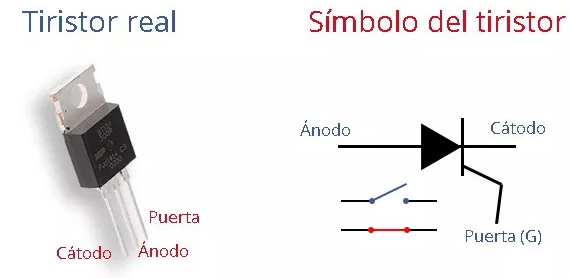
\includegraphics[scale=0.5]{Pictures/Tiristor.PNG}
\caption{Tiristor y su estructura}
\end{figure}

Funcionamiento.\\
Los tiristores están conformados por 3 terminales un ánodo, un cátodo y una compuerta o mejor conocida “gate”, su funcionamiento se asemeja al de un relevador o un interruptor mecánico, Ya que cuando aplicas una corriente a la terminal gate este se activa y obtiene la característica de dejar pasar a la electricidad.
\begin{figure}[hbtp]
\centering
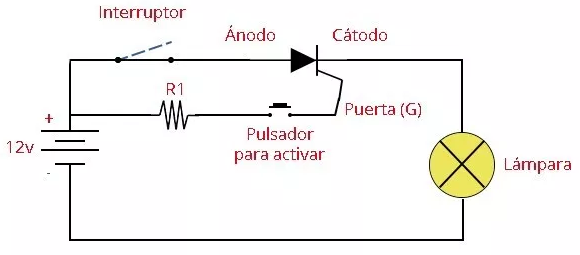
\includegraphics[scale=0.6]{Pictures/Circuito.PNG}
\caption{Circuito con tiristor}
\end{figure}

Control de fase con tiristor.\\
Un SCR se usa principalmente para controlar la potencia que se entrega a una carga. (en el caso de la figura es un bombillo o foco). La fuente de voltaje puede ser 120 / 240 VCA , etc. La potencia suministrada a la carga se controla variando el ángulo de conducción. El circuito RC produce un corrimiento de la fase entre la tensión de entrada y la tensión en el condensador que es la que suministra la corriente a la compuerta del tiristor.
\begin{figure}[hbtp]
\centering
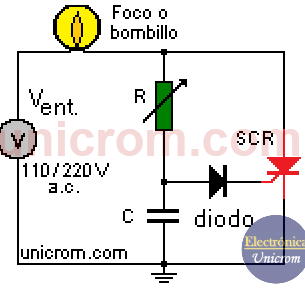
\includegraphics[scale=0.5]{Pictures/Control.PNG}
\caption{Circuito de control de fase con tiristor}
\end{figure}
\footnote{Universidad Politécnica de la Zona Metropolitana de Guadalajara}

\newpage
Como R es un potenciómetro, el valor resistivo puede variar y así producir un corrimiento de fase ajustable, que causará que la entrega de potencia a la carga (el bombillo) también sea variable. Con ésto se logra que la intensidad de la luz en el bombillo varíe.\\

El diodo en la compuerta del tiristor se usa para bloquear la tensión de compuerta durante el ciclo negativo (de 180$^{\circ}$ a 360$^{\circ}$). Formas de onda de la señal de entrada y en la carga para diferentes corrimientos de fase.\\
\begin{figure}[hbtp]
\centering
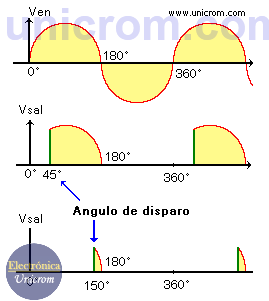
\includegraphics[scale=0.7]{Pictures/Ondas.PNG}
\caption{Señal de onda}
\end{figure}

\begin{itemize}
\item El 1er diagrama muestra la onda de entrada. Observar los ptos. 0$^{\circ}$, 180$^{\circ}$ y 360$^{\circ}$.
\item El 2do diagrama muestra la señal aplicada a la carga cuando el disparo es a los 45$^{\circ}$.
\item El 3er diagrama muestra la señal aplicada a la carga cuando el disparo es a los 150$^{\circ}$.
\end{itemize}

En el segundo y tercer diagrama se ve que la semi-onda negativa ha desaparecido, y esto es debido a que el SCR se comporta, cuando está conduciendo, como un diodo común. El área bajo la curva en el segundo y tercer diagrama representa la energía transferida a la carga.

El segundo diagrama tiene un área bajo la curva mayor, entonces indica que, en este caso, hay más energía entregada al bombillo que en el tercer diagrama.

El máximo corrimiento de fase se logra cuando el potenciómetro tiene su mayor valor y el mínimo cuando este tiene su valor más pequeño. Ver que cuando R = 0 (valor mínimo del potenciómetro) el capacitor está en paralelo con el tiristor y éste se comporta prácticamente como un diodo, pues se dispara casi inmediatamente que la señal de entrada es 0$^{\circ}$.
\footnote{Universidad Politécnica de la Zona Metropolitana de Guadalajara}

\newpage
\section{Materiales}
\begin{itemize}
\item Protoboard
\item Cable para protoboard
\item Capacitor 1 $\mu$F
\item Potenciómetro 500K$\Omega$
\item Resistencia 1K$\Omega$
\item TRIAC BT138
\item DIC 
\item Foco 110V 
\item Clavija
\end{itemize}

\section{Desarrollo}
\subsection{Primero armaremos el siguiente circuito tanto a alguna aplicación para simularlo como en protoboard para probar que funciona físicamente y lo realiza correctamente.}
\begin{figure}[hbtp]
\centering
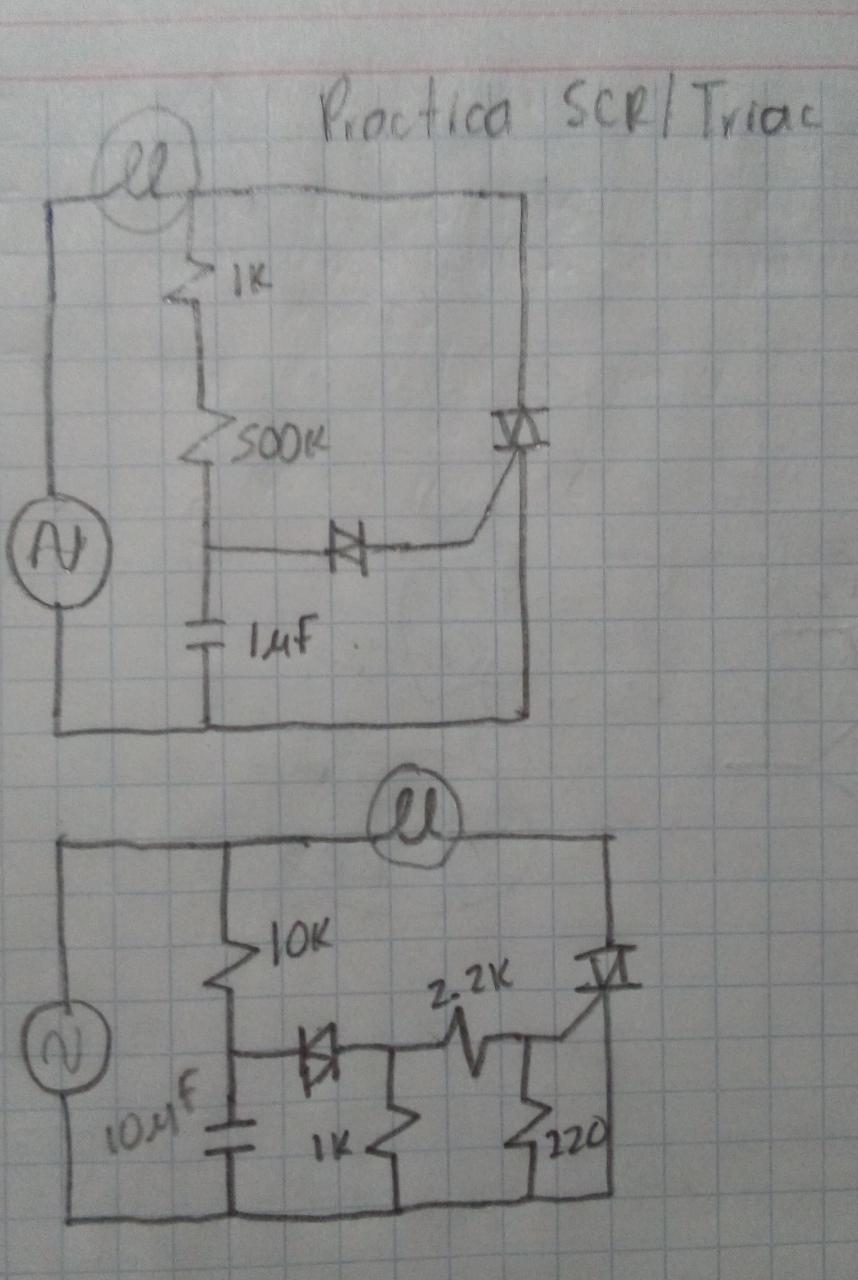
\includegraphics[scale=0.2]{Pictures/Circuitos.jpeg}
\caption{Circuitos de control de fase y corriente con tiristor}
\end{figure}
Escogemos alguno de los dos circuitos para armarlo en protoboard y el otro simularlo como requisito para entregar.

\footnote{Universidad Politécnica de la Zona Metropolitana de Guadalajara}

\newpage
\subsection{Armamos el circuito en Proteus quedando:}
\begin{figure}[hbtp]
\centering
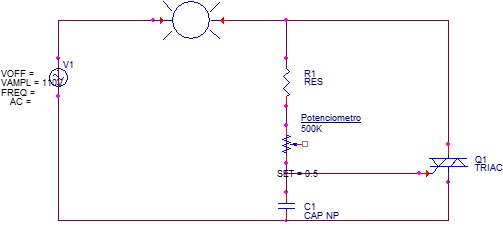
\includegraphics[scale=0.7]{Pictures/CIRCUITO.jpg}
\caption{Simulación circuito de control}
\end{figure}

\subsection{Una vez armado el circuito vamos a enchufar todo como corresponde teniendo en cuenta que debemos conectar la clavija de manera correcta, sabiendo cual es el agujero del contacto positivo o que tiene mas voltaje, esto se logra con el multímetro, midiendo voltaje colocando las puntas dentro del contacto.}
Al momento de enchufar la clavija debes tomar en cuenta que estés colocando el positivo que tomaste de tu circuito en el positivo del contacto de luz, para no tener problemas a la hora de conectarlo.

\subsection{Mueve el potenciómetro hasta el tope y comienza a subirle al potenciómetro y observa lo que sucede.}
Al momento de ir subiéndole al potenciómetro se observa que va incrementando la intensidad de la luz, teniendo 3 fases: apagado completamente, medio encendido y encendido completamente.

\footnote{Universidad Politécnica de la Zona Metropolitana de Guadalajara}

\newpage
\section{Conclusiones}
Luis Osvaldo Cervantes Martínez.\\
En este circuito me permitio de manera muy sencilla el funcionamiento de un Dimmer, en el cual me pude percatar de la gran inportancia del triac para esta ocasión, ya que este funciona o puede funcionar como un atenuador de focos incandecentes y como un regulador de velocidad, lo que me permitio conocer y aprender el funcinamiento de este mismo.\\\\

Ulises Isaac Reyes Alvarez.\\
Para este circuito tuvimos problemas al resolverlo ya que algunas partes del circuito estaban mal, se tuvo que corregir y volver a armar correctamente, una vez teniendolo fue demasiado fácil la realización de la practica. Me gusto el realizarla ya que con ella me dio muchas ideas para hacer en algun lado, ya que al subir el potenciómetro podemos generar la intensidad de luz que ocupemos haciendo un poco mas bonita la noche al iluminarla de esa manera.\\
Aprendimos a utilizar los DIACs y la activación de los TRICs, mediante sus datasheet's.

\footnote{Universidad de la Zona Metropolitana de Guadalajara}

\newpage
\section{Referencias bibliográficas}
\url{https://unicrom.com/tiristor-scr-en-corriente-alterna/}\\\\
\url{https://www.ingmecafenix.com/electronica/que-es-un-tiristor-y-como-funciona/}











\end{document}